\documentclass[11pt, letterpaper]{article}
\usepackage[utf8]{inputenc}
\usepackage[margin=1in]{geometry}
\usepackage{amsmath}
\usepackage{amssymb}
\usepackage{tikz}
\usepackage{pgfplots}
\pgfplotsset{compat=1.18}
\usetikzlibrary{patterns, arrows.meta, decorations.pathreplacing, calc, positioning}
\usepackage{float}
\usepackage{enumitem}
\usepackage{titlesec}

\setlength{\parindent}{0pt}
\setlength{\parskip}{0.5em}

% Title Formatting
\titleformat{\section}{\large\bfseries}{\thesection}{1em}{}
\titleformat{\subsection}{\normalsize\bfseries}{\thesubsection}{1em}{}

% Meta Data
\title{\textbf{ECON 315: International Economics \\ Problem Set \#3}}
\author{Sean Balbale \\ Trinity College (Class of '27)}
\date{April 20, 2026}

\begin{document}

\maketitle

\section*{Problem 1}

\textbf{Restatement:} Suppose that the domestic demand and supply curve for towels in Guatemala is given by:
\[
  P = 66 - 2Q \quad \text{(demand)}, \qquad P = 6 + Q \quad \text{(supply)},
\]
where $P$ and $Q$ denote price (in pesos) and quantity (in towels), respectively. Assume a one-to-one peso--dollar exchange rate throughout.

\subsection*{(a) What is the autarchy price of towels and the quantity produced?}
\noindent \textbf{Solution:} Set quantity demanded equal to quantity supplied ($Q_d = Q_s$):
\[
  66 - 2Q = 6 + Q \;\Longrightarrow\; 60 = 3Q \;\Longrightarrow\; Q_A = \mathbf{20 \text{ towels}}.
\]
Substituting back, $P_A = 6 + 20 = \mathbf{26 \text{ pesos}}$.

\subsection*{(b) What are the levels of domestic production, consumption, and imports if the world price is \$20?}
\noindent \textbf{Solution:} Since $P_W = 20 < P_A = 26$, Guatemala is a net importer.
\begin{itemize}
  \item Domestic production: $20 = 6 + Q_s \;\Longrightarrow\; Q_s = \mathbf{14 \text{ towels}}$.
  \item Domestic consumption: $20 = 66 - 2Q_d \;\Longrightarrow\; 2Q_d = 46 \;\Longrightarrow\; Q_d = \mathbf{23 \text{ towels}}$.
  \item Imports: $Q_d - Q_s = 23 - 14 = \mathbf{9 \text{ towels imported}}$.
\end{itemize}

\subsection*{(c) How do your answers in part b change if this country were to impose a tariff of 10 percent? Show this graphically.}
\noindent \textbf{Solution:} Guatemala is small, so the tariff passes through fully to the domestic price: $P_T = 20 \times 1.10 = \mathbf{\$22}$.
\begin{itemize}
  \item Domestic production: $22 = 6 + Q_s' \;\Longrightarrow\; Q_s' = \mathbf{16 \text{ towels}}$.
  \item Domestic consumption: $22 = 66 - 2Q_d' \;\Longrightarrow\; 2Q_d' = 44 \;\Longrightarrow\; Q_d' = \mathbf{22 \text{ towels}}$.
  \item Imports: $Q_d' - Q_s' = 22 - 16 = \mathbf{6 \text{ towels imported}}$.
\end{itemize}

\noindent The tariff raises domestic production by 2 towels, contracts consumption by 1 towel, and cuts imports by 3 towels relative to free trade.

\begin{figure}[H]
  \centering
  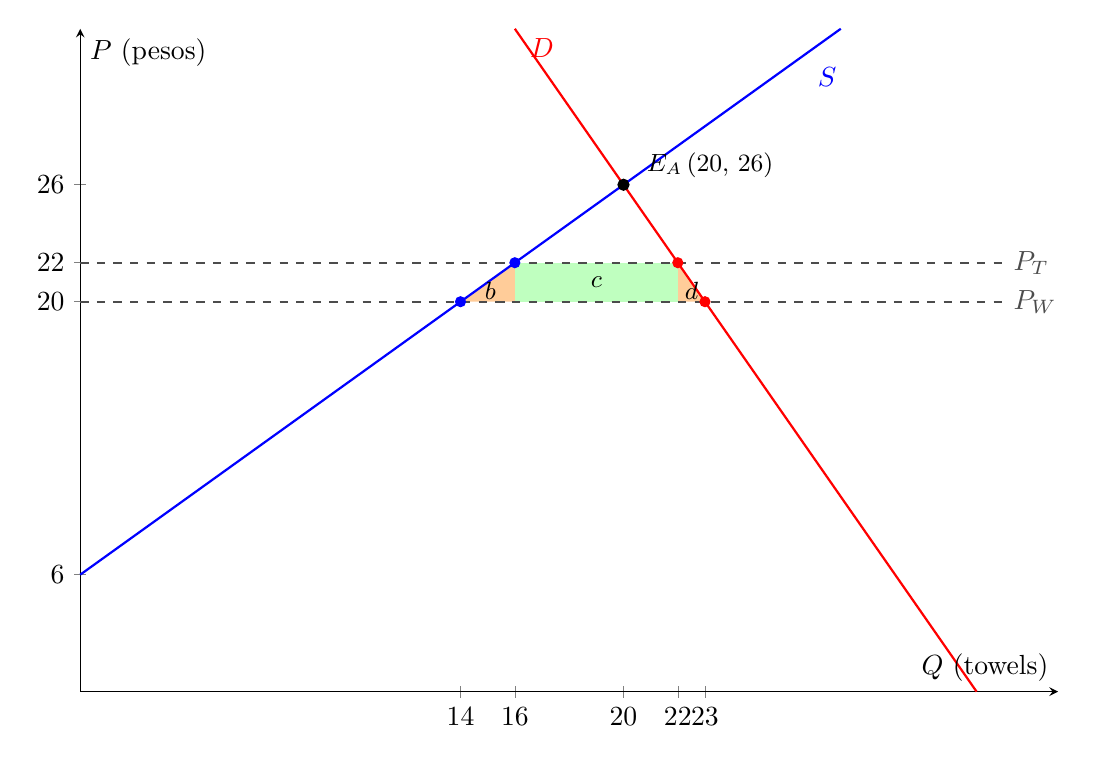
\begin{tikzpicture}
    \begin{axis}[
        axis lines = middle,
        xlabel = {$Q$ (towels)},
        ylabel = {$P$ (pesos)},
        xmin = 0, xmax = 36, ymin = 0, ymax = 34,
        xtick = {14, 16, 20, 22, 23},
        ytick = {6, 20, 22, 26},
        width = 14cm, height = 10cm,
        clip = false,
      ]

      % DWL triangles (shaded orange)
      \path[fill=orange!40, draw=none] (axis cs:14,20) -- (axis cs:16,20) -- (axis cs:16,22) -- cycle;
      \path[fill=orange!40, draw=none] (axis cs:22,20) -- (axis cs:23,20) -- (axis cs:22,22) -- cycle;
      % Tariff revenue rectangle (shaded green)
      \path[fill=green!25, draw=none] (axis cs:16,20) -- (axis cs:22,20) -- (axis cs:22,22) -- (axis cs:16,22) -- cycle;

      % Supply curve: P = 6 + Q
      \addplot[thick, blue, domain=0:28] {6 + x};
      \node[blue] at (axis cs:27.5, 31.5) {$S$};
      % Demand curve: P = 66 - 2Q
      \addplot[thick, red, domain=16:33] {66 - 2*x};
      \node[red] at (axis cs:17, 33) {$D$};

      % World price line
      \addplot[dashed, thick, black!70, domain=0:34] {20};
      \node[anchor=west, black!70] at (axis cs:34,20) {$P_W$};
      % Tariff-inclusive price line
      \addplot[dashed, thick, black!70, domain=0:34] {22};
      \node[anchor=west, black!70] at (axis cs:34,22) {$P_T$};

      % Autarky point
      \filldraw[black] (axis cs:20,26) circle [radius=2pt];
      \node[anchor=west, font=\small] at (axis cs:20.5, 27) {$E_A\,(20,\,26)$};

      % Key points
      \filldraw[blue] (axis cs:14,20) circle [radius=1.8pt];
      \filldraw[blue] (axis cs:16,22) circle [radius=1.8pt];
      \filldraw[red]  (axis cs:23,20) circle [radius=1.8pt];
      \filldraw[red]  (axis cs:22,22) circle [radius=1.8pt];

      % Labels inside shaded regions
      \node[font=\small] at (axis cs:15.1, 20.55) {$b$};
      \node[font=\small] at (axis cs:22.5, 20.55) {$d$};
      \node[font=\small] at (axis cs:19, 21) {$c$};

    \end{axis}
  \end{tikzpicture}
  \caption{Tariff effects in Guatemala. Free-trade imports $= 23-14=9$; tariff imports $= 22-16=6$. Triangle $b$ is the production-distortion loss; triangle $d$ is the consumption-distortion loss; rectangle $c$ is tariff revenue.}
\end{figure}

\subsection*{(d) In peso terms, what are the deadweight costs of the tariff?}
\noindent \textbf{Solution:} The deadweight loss (DWL) consists of two triangles in the diagram above:
\[
  \underbrace{\text{Production distortion ($b$):}}_{\text{area} = \tfrac{1}{2}(\Delta Q_s)(\Delta P)} = \tfrac{1}{2}(16-14)(22-20) = \mathbf{2 \text{ pesos}},
\]
\[
  \underbrace{\text{Consumption distortion ($d$):}}_{\text{area} = \tfrac{1}{2}(\Delta Q_d)(\Delta P)} = \tfrac{1}{2}(23-22)(22-20) = \mathbf{1 \text{ peso}}.
\]
\[
  \text{Total DWL} = b + d = \mathbf{3 \text{ pesos}}.
\]

\subsection*{(e) How much revenue does the government raise from the tariff?}
\noindent \textbf{Solution:} Revenue is the per-unit tariff times the number of units imported under the tariff:
\[
  \text{Revenue} = (P_T - P_W) \times \text{Imports}_T = \$2 \times 6 = \mathbf{12 \text{ pesos}}.
\]

\subsection*{(f) Would the deadweight cost of the tariff be greater or smaller if the price elasticity of demand and/or supply is less elastic? Explain.}
\noindent \textbf{Solution:} The DWL would be \textbf{smaller}. The two triangles have area $\tfrac{1}{2}(\Delta Q)(\Delta P)$; while the price wedge $\Delta P$ is fixed by the tariff, $\Delta Q$ is governed by the slope of the relevant curve. A less-elastic (steeper) curve means quantity responds less to the price change, which shrinks the base of the DWL triangle.

\subsection*{(g) If, instead of Guatemala, this was a large country, what impact would the imposition of a tariff have on the world price for towels? Would the nation's terms of trade improve? Under what conditions? Explain.}
\noindent \textbf{Solution:} If Guatemala were large, the tariff would reduce its import demand enough to move the world price. Because foreign exporters face a smaller market, they must accept a lower price to clear the residual quantity; the world price of towels, $P_W$, \textbf{falls}.

Guatemala's terms of trade (export prices over import prices) therefore \textbf{improve}, because towels are an import and the import price has fallen. The net welfare effect is positive only if the terms-of-trade gain (extracting revenue from foreign exporters) is larger than the volume-of-trade loss (the deadweight loss), assuming trade partners do not retaliate.

\vspace{1em}
\section*{Problem 2}

\textbf{Restatement:} Show how transportation costs between two countries can be analyzed using supply and demand diagrams. Assume that the free trade price for the two countries is \$6 per unit of wheat and that the autarchy prices (before trade) are \$3 and \$9 for country A and B, respectively. Explain the relationship between the equilibrium price, supply and demand for the two countries? Now, suppose country A has a more inelastic set of demand and/or supply curves relative to Country B. Where would the burden of the \$1 transportation cost fall more heavily, and why?

\subsection*{Setup and the wedge created by transport costs}
\noindent \textbf{Solution:} Because $P_A^{\text{autarky}} = \$3 < P_B^{\text{autarky}} = \$9$, country A has comparative advantage in wheat and exports to country B. Under free trade \textit{without} transport cost, the world price settles at \$6 in both countries. A transport cost of \$1 drives a wedge between the price received by A's producers and the price paid by B's consumers:
\[
  P_B - P_A = \$1, \qquad \text{and with equal sharing,}\qquad P_A = \$5.50,\quad P_B = \$6.50.
\]

\begin{figure}[H]
  \centering
  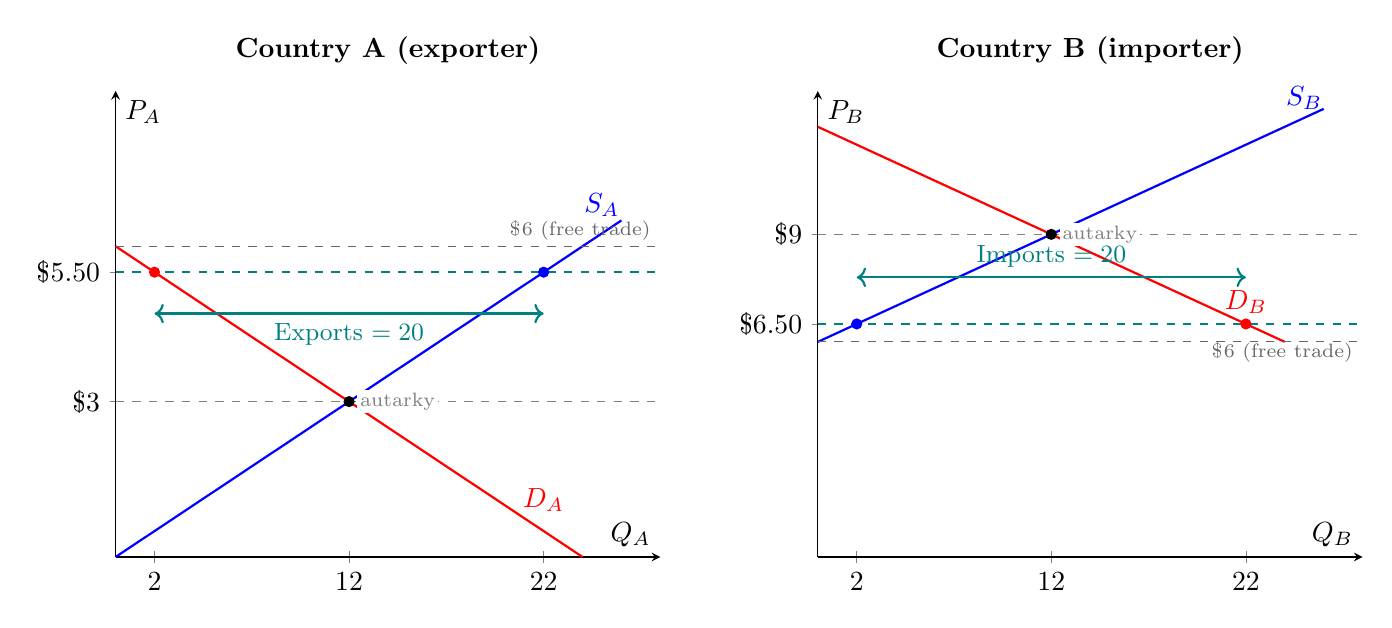
\begin{tikzpicture}
    % ---------- Country A (exporter) ----------
    \begin{axis}[
        name = plotA,
        title = {\textbf{Country A (exporter)}},
        axis lines = middle,
        xlabel = {$Q_A$}, ylabel = {$P_A$},
        xmin = 0, xmax = 28, ymin = 0, ymax = 9,
        xtick = {2, 12, 22}, ytick = {3, 5.5},
        yticklabels = {\$3, \$5.50},
        width = 8.5cm, height = 7.5cm,
        clip = false,
      ]
      \addplot[thick, blue, domain=0:26] {x/4};
      \node[blue] at (axis cs:25, 6.8) {$S_A$};
      \addplot[thick, red, domain=0:24]  {6 - x/4};
      \node[red] at (axis cs:22, 1.1) {$D_A$};

      \addplot[dashed, gray, domain=0:28] {3};
      \addplot[dashed, black!60, domain=0:28] {6};
      \node[anchor=east, font=\scriptsize, black!60] at (axis cs:28, 6.3) {\$6 (free trade)};
      \addplot[dashed, teal, thick, domain=0:28] {5.5};

      \filldraw[black] (axis cs:12,3) circle [radius=1.8pt];
      \node[anchor=west, font=\scriptsize, gray, fill=white, inner sep=1pt] at (axis cs:12.4, 3) {autarky};

      \filldraw[red]  (axis cs:2,5.5)  circle [radius=1.8pt];
      \filldraw[blue] (axis cs:22,5.5) circle [radius=1.8pt];

      \draw[<->, teal, thick] (axis cs:2, 4.7) -- (axis cs:22, 4.7)
      node[midway, below, teal, font=\small] {Exports $= 20$};
    \end{axis}

    % ---------- Country B (importer) ----------
    \begin{axis}[
        name = plotB,
        at = {($(plotA.east)+(2cm,0)$)}, anchor = west,
        title = {\textbf{Country B (importer)}},
        axis lines = middle,
        xlabel = {$Q_B$}, ylabel = {$P_B$},
        xmin = 0, xmax = 28, ymin = 0, ymax = 13,
        xtick = {2, 12, 22}, ytick = {6.5, 9},
        yticklabels = {\$6.50, \$9},
        width = 8.5cm, height = 7.5cm,
        clip = false,
      ]
      \addplot[thick, blue, domain=0:26] {6 + x/4};
      \node[blue] at (axis cs:25, 12.8) {$S_B$};
      \addplot[thick, red, domain=0:24]  {12 - x/4};
      \node[red] at (axis cs:22, 7.1) {$D_B$};

      \addplot[dashed, gray, domain=0:28] {9};
      \addplot[dashed, black!60, domain=0:28] {6};
      \node[anchor=east, font=\scriptsize, black!60] at (axis cs:28, 5.7) {\$6 (free trade)};
      \addplot[dashed, teal, thick, domain=0:28] {6.5};

      \filldraw[black] (axis cs:12,9) circle [radius=1.8pt];
      \node[anchor=west, font=\scriptsize, gray, fill=white, inner sep=1pt] at (axis cs:12.4, 9) {autarky};

      \filldraw[blue] (axis cs:2,6.5)  circle [radius=1.8pt];
      \filldraw[red]  (axis cs:22,6.5) circle [radius=1.8pt];

      \draw[<->, teal, thick] (axis cs:2, 7.8) -- (axis cs:22, 7.8)
      node[midway, above, teal, font=\small] {Imports $= 20$};
    \end{axis}
  \end{tikzpicture}
  \caption{With a \$1 transport cost split evenly, A receives \$5.50 and B pays \$6.50. The market clears where Exports = Imports.}
\end{figure}

\subsection*{What does equal sharing assume about elasticities?}
\noindent \textbf{Solution:} Equal sharing requires that A's excess-supply curve and B's excess-demand curve are \textit{equally elastic} at the trading equilibrium.

\subsection*{Incidence when A has more-inelastic curves than B}
\noindent \textbf{Solution:} If A's supply and demand are more inelastic than B's, then \textbf{the burden falls more heavily on country A}. The less-responsive side of the market bears more of the wedge. A's producers cannot easily divert resources if prices fall, and A's consumers cannot easily substitute away if prices rise. When the transport cost drives prices apart, A must absorb most of the adjustment to keep B (who has highly elastic alternatives) buying its exports.

\vspace{1em}
\section*{Problem 3}

\textbf{Restatement:} In class we discussed the difference between nominal and effective protection. Answer the following questions pertaining to the effective rate of protection ($g$). The equation is:
\[
  g = \frac{t_f - a\, t_i}{1 - a}
\]

\subsection*{(a) Show that if no imported inputs go into domestic production of the final good, then $g$ is equal to the nominal tariff rate on the final good ($t_f$).}
\noindent \textbf{Solution:} Substituting $a = 0$ into the formula:
\[
  g = \frac{t_f - (0)\,t_i}{1 - 0} = \frac{t_f}{1} = \mathbf{t_f}.
\]
\textit{Interpretation:} When domestic production uses no imported inputs, the entire product price is domestic value added. The nominal tariff is therefore equivalent to the effective rate.

\subsection*{(b) Suppose that $t_f = 0.5$, $t_i = 0.2$, and $a = 0.4$. Find the $g$ given to the domestic producers of this commodity and interpret in words.}
\noindent \textbf{Solution:}
\[
  g = \frac{0.5 - (0.4)(0.2)}{1 - 0.4} = \frac{0.5 - 0.08}{0.6} = \frac{0.42}{0.6} = \mathbf{0.70 \text{ or } 70\%}.
\]
\textit{Interpretation:} Although the nominal tariff on the final good is only 50\%, domestic producers enjoy effective protection of 70\% on their value-added activities because the input tariff ($20\%$) is lower than the output tariff, sheltering domestic value added by a magnified amount.

\subsection*{(c) Given that $a = 0.5$ and $t_f = 0.4$, find $g$ when $t_i = 0.8$, and $t_i = 1.0$. In both cases, explain the nature of your results.}
\noindent \textbf{Solution:}
\begin{itemize}
  \item \textbf{When $t_i = 0.8$:}
    \[
      g = \frac{0.4 - (0.5)(0.8)}{1 - 0.5} = \frac{0.4 - 0.4}{0.5} = \mathbf{0\%}.
    \]
    Effective protection is \textit{zero}---the heavy tax on imported inputs exactly offsets the output tariff.

  \item \textbf{When $t_i = 1.0$:}
    \[
      g = \frac{0.4 - (0.5)(1.0)}{1 - 0.5} = \frac{-0.1}{0.5} = \mathbf{-20\%}.
    \]
    Effective protection is \textit{negative}---the tariff structure actively penalizes domestic producers by raising input costs more than revenue.
\end{itemize}

\subsection*{(d) What are the main drawbacks (at least two) of the concept of effective protection? Explain fully.}
\noindent \textbf{Solution:}
\begin{itemize}
  \item \textit{Fixed input-output coefficients:} The formula assumes $a$ is technologically constant, ignoring dynamic substitution between imported and domestic inputs when relative prices change.
  \item \textit{Partial-equilibrium assumption:} It looks at one industry in isolation, ignoring general-equilibrium effects (like exchange rate shifts) and completely ignores non-tariff barriers.
\end{itemize}

\vspace{1em}
\section*{Problem 4}

\textbf{Restatement:} Carefully identify and discuss the conditions which can lead to Bhagwati's ``immiserizing growth'' concept. Which type of growth is most likely to lead to a decline in the nation's welfare, and why? How is this concept related to Prebisch's argument concerning the deterioration in the net barter terms of trade? A general equilibrium graph is needed.

\subsection*{The conditions for immiserizing growth}
\noindent \textbf{Solution:} Immiserizing growth is the counterintuitive case where a country's economic growth leaves the country \textit{worse off} in welfare terms. The outcome requires four conditions:
\begin{enumerate}
  \item \textbf{Large-country status:} The country must be large enough to affect world prices.
  \item \textbf{Export-biased growth:} Growth must be disproportionately concentrated in the export sector.
  \item \textbf{Inelastic foreign demand:} Foreigners' demand for the country's exports must be highly price-inelastic.
  \item \textbf{Trade dependence:} The country's trade must represent a large share of its economy.
\end{enumerate}

\noindent The type of growth most likely to trigger this is \textbf{export-biased growth}. When a large nation massively expands its export sector, it floods the global market. Because foreign demand is inelastic, the nation must drastically slash prices to sell its surplus. The terms-of-trade loss exceeds the real income gain from the expanded PPF, pushing the nation to a lower community indifference curve.

\begin{figure}[H]
  \centering
  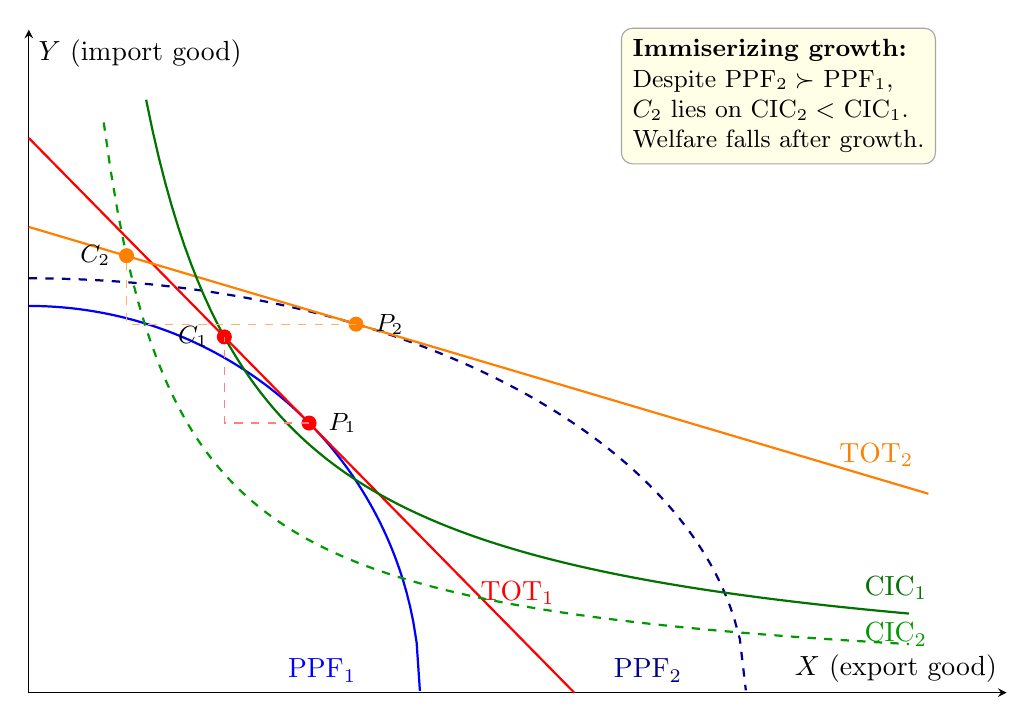
\begin{tikzpicture}
    \begin{axis}[
        axis lines = middle,
        xlabel = {$X$ (export good)}, ylabel = {$Y$ (import good)},
        xmin = 0, xmax = 15, ymin = 0, ymax = 12,
        xtick = \empty, ytick = \empty,
        width = 14cm, height = 10cm,
        clip = false,
        samples = 120,
      ]

      % ---- PPF_1: X²/36 + Y²/49 = 1, so Y = 7·sqrt(1 - X²/36)
      \addplot[thick, blue, domain=0:6] {7 * sqrt(1 - x*x/36)};
      \node[blue] at (axis cs:4.5, 0.4) {PPF$_1$};

      % ---- PPF_2: X²/121 + Y²/56.25 = 1, so Y = 7.5·sqrt(1 - X²/121)
      \addplot[thick, blue!55!black, dashed, domain=0:11] {7.5 * sqrt(1 - x*x/121)};
      \node[blue!55!black] at (axis cs:9.5, 0.4) {PPF$_2$};

      % ---- TOT_1: Y = 10.04 - 1.2X (through P_1 = (4.30, 4.88))
      \addplot[thick, red, domain=0:8.37] {10.04 - 1.2*x};
      \node[red] at (axis cs:7.5, 1.8) {TOT$_1$};

      % ---- TOT_2: Y = 8.43 - 0.35X
      \addplot[thick, orange, domain=0:13.8] {8.43 - 0.35*x};
      \node[orange] at (axis cs:13, 4.3) {TOT$_2$};

      % ---- CIC_1: XY = 19.32 (through C_1 = (3.0, 6.44))
      \addplot[thick, green!45!black, domain=1.8:13.5] {19.32/x};
      \node[green!45!black] at (axis cs:13.3, 1.9) {CIC$_1$};

      % ---- CIC_2: XY = 11.87 (through C_2 = (1.5, 7.91))
      \addplot[thick, green!60!black, dashed, domain=1.15:13.5] {11.87/x};
      \node[green!60!black] at (axis cs:13.3, 1.05) {CIC$_2$};

      % ---- Production points (on PPFs, tangent to TOT lines)
      \filldraw[red]    (axis cs:4.30, 4.88) circle [radius=2.5pt];
      \node[anchor=west, font=\small] at (axis cs:4.45, 4.88) {$P_1$};

      \filldraw[orange] (axis cs:5.02, 6.67) circle [radius=2.5pt];
      \node[anchor=west, font=\small] at (axis cs:5.17, 6.67) {$P_2$};

      % ---- Consumption points (on TOTs, tangent to CICs)
      \filldraw[red]    (axis cs:3.0, 6.44) circle [radius=2.5pt];
      \node[anchor=east, font=\small] at (axis cs:2.9, 6.44) {$C_1$};

      \filldraw[orange] (axis cs:1.5, 7.91) circle [radius=2.5pt];
      \node[anchor=east, font=\small] at (axis cs:1.4, 7.91) {$C_2$};

      % ---- Trade triangles (thin dashed guides)
      \draw[dashed, red!50, thin]    (axis cs:4.30, 4.88) -- (axis cs:3.0, 4.88) -- (axis cs:3.0, 6.44);
      \draw[dashed, orange!60, thin] (axis cs:5.02, 6.67) -- (axis cs:1.5, 6.67) -- (axis cs:1.5, 7.91);

      % ---- Callout box (positioned upper-right to avoid other content)
      \node[font=\small, align=left, draw=black!35, fill=yellow!10, rounded corners, inner sep=4pt]
      at (axis cs:11.5, 10.8) {
        \textbf{Immiserizing growth:}\\
        Despite PPF$_2 \succ$ PPF$_1$, \\
        $C_2$ lies on CIC$_2 <$ CIC$_1$.\\
        Welfare falls after growth.
      };

    \end{axis}
  \end{tikzpicture}
  \caption{Bhagwati's immiserizing growth. The PPF expands outward in an export-biased way (PPF$_1 \to$ PPF$_2$), but inelastic foreign demand collapses the terms of trade (TOT$_1 \to$ TOT$_2$). Consumption shifts from $C_1$ to $C_2$, meaning welfare falls after growth.}
\end{figure}

\subsection*{Connection to Prebisch's terms-of-trade deterioration thesis}
\noindent \textbf{Solution:} Prebisch argued that developing countries specializing in primary-commodity exports face a long-run tendency for their net barter terms of trade to deteriorate. This is because raw commodities face inelastic global demand while manufactured imports face elastic demand. If developing nations experience export-biased growth in primary commodities, they inadvertently trigger Bhagwati's immiserizing growth mechanism---flooding the market and crashing their own export prices relative to the manufactured goods they import.

\end{document}
